%\part{Spezifikation}

\chapter{Kapitel}

Im Folgenden werden die Use-Case-Diagramme des \SECH-Browsers übersichtlich vorgestellt. Diese veranschaulichen alle verschiedenen Funktionalitäten, die der Benutzer tätigen kann.

\section{Menüführung des Browsers Teil 1}

\begin{figure}[htb]
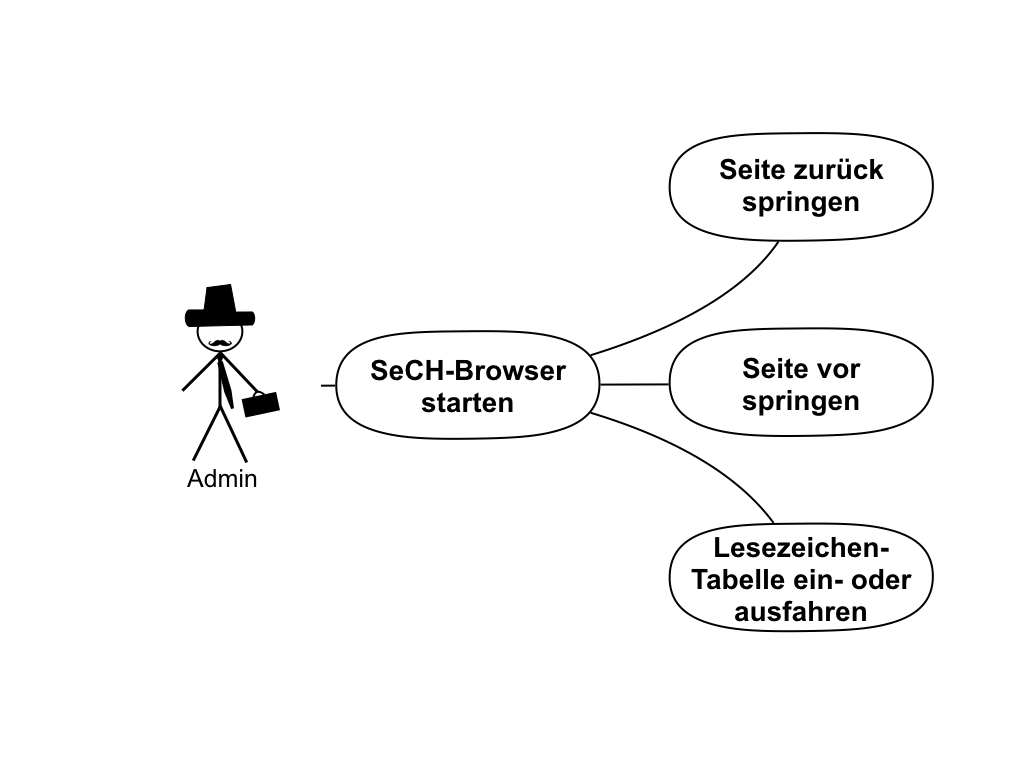
\includegraphics[width=\textwidth]{Use-Case-Diagramme_001.png}
	\caption{Use--Case--Diagramm --- Menüführung Teil 1}
	\label{fig:Menüführung Teil 1}
\end{figure}
	
Dieses Use-Case-Diagramm zeigt die wesentlichen Funktionen des Browsers an. Der Nutzer kann auf einer Homepage eine Seite zurück- und vorspringen. Weiterhin hat er die Möglichkeit die Lesezeichen-Tabelle auszufahren und im Anschluss diese wieder einzufahren.

\section{Lesezeichenverwaltung des Browsers}

\begin{figure}[htb]
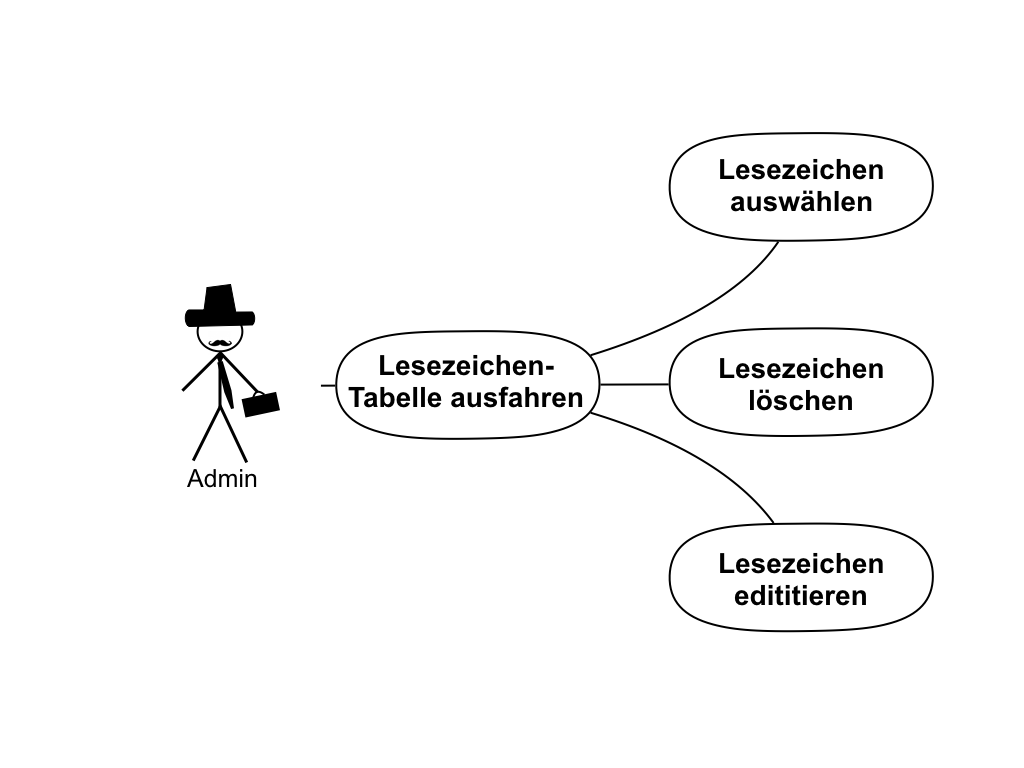
\includegraphics[width=\textwidth]{Use-Case-Diagramme_002.png}
	\caption{Use--Case--Diagramm --- Lesezeichenverwaltung}
	\label{fig:Lesezeichenverwaltung}
\end{figure}

Ist die Lesezeichen-Tabelle ausgefahren, so kann der Benutzer ein persönlich angelegtes Lesezeichen anklicken und es wird die von ihm gewünschte Seite geladen. Das Löschen und das Editieren ausgewählter Lesezeichen ist ebenfalls in der Tabelle verwirklichbar.

\section{Menüführung des Browsers Teil 2}

\begin{figure}[htb]
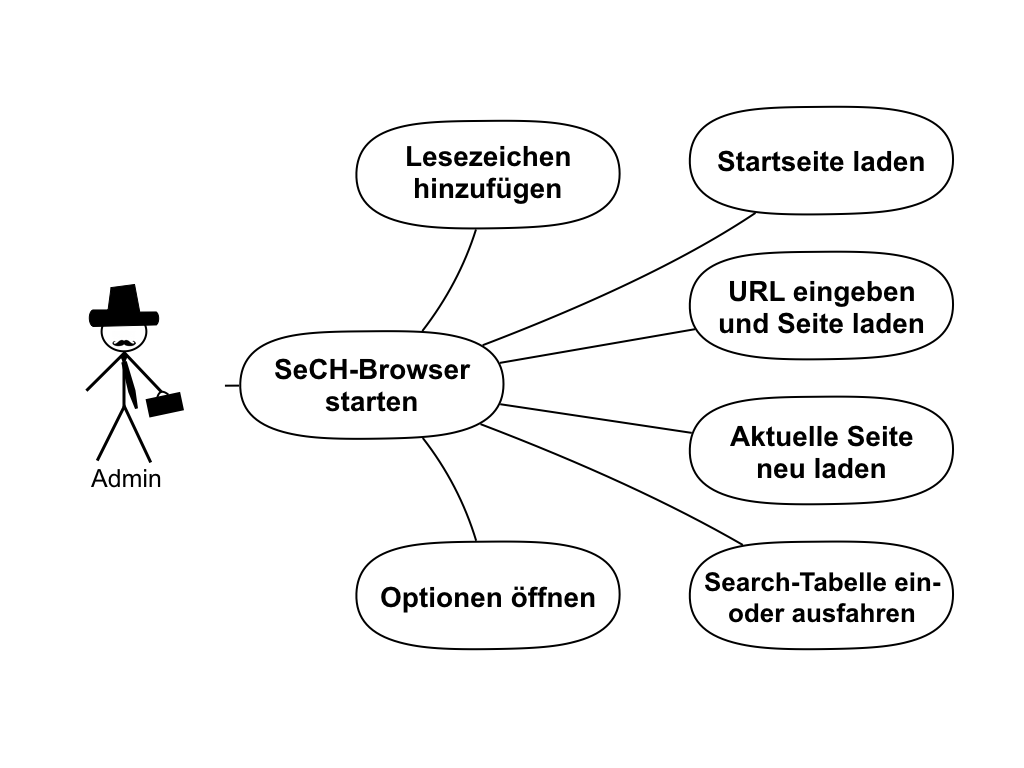
\includegraphics[width=\textwidth]{Use-Case-Diagramme_003.png}
	\caption{Use--Case--Diagramm --- Menüführung Teil 2}
	\label{fig:Menüführung Teil 2}
\end{figure}
In diesem Use-Case Diagramm werden weitere Navigationselemente des Browsers vorgestellt. Der Nutzer kann eigene Lesezeichen hinzufügen, die von ihm definierte Startseite laden, eine URL in die Address-Bar eingeben und diese dann laden, die aktuelle Seite neu laden, die \SEARCH-Tabelle aus- und einfahren und das Fenster für Optionen öffnen.

\section{\SEARCH--Tagverwaltung des Browsers}
\begin{figure}[htb]
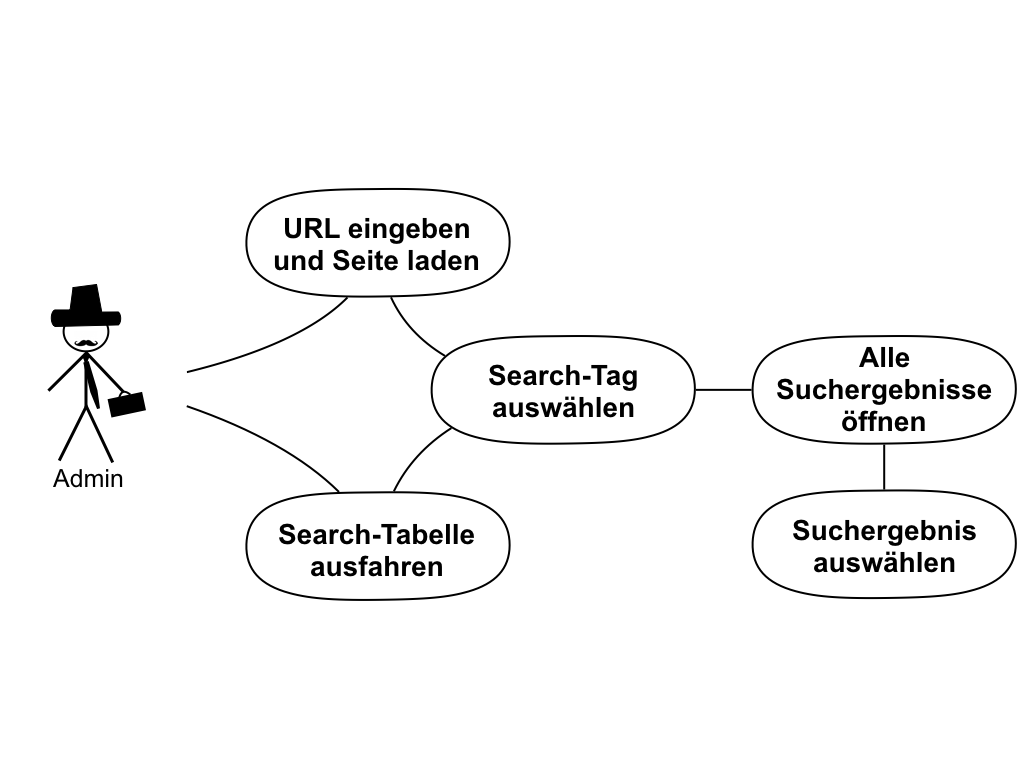
\includegraphics[width=\textwidth]{Use-Case-Diagramme_004.png}
	\caption{Use--Case--Diagramm --- \SEARCH--Tagverwaltung}
	\label{fig:SEARCH-Tagverwaltung}
\end{figure}
Der Nutzer kann durch zwei verschiedene Wege Suchergebnisse für das gewünschte \SEARCH-Tag anzeigen lassen. Zunächst muss der Nutzer durch Eingabe und Bestätigung einer URL die Seite aufrufen. Die erste Variante ist das gewünschte \SEARCH-Tag, welches hervorgehoben wird, anzuklicken. Die zweite Variante ist durch Ausfahren der \SEARCH-Tabelle das gewünschte \SEARCH-Tag auszuwählen. Beide Wege führen zum selben Ergebnis, und zwar die Anzeige des ersten Suchergebnisses des jeweiligen \SEARCH-Tags. Zusätzlich kann der Nutzer alle weitere Suchergebnisse zu einem \SEARCH-Tag anzeigen lassen.

\section{Browser-Einstellungen}
\begin{figure}[htb]
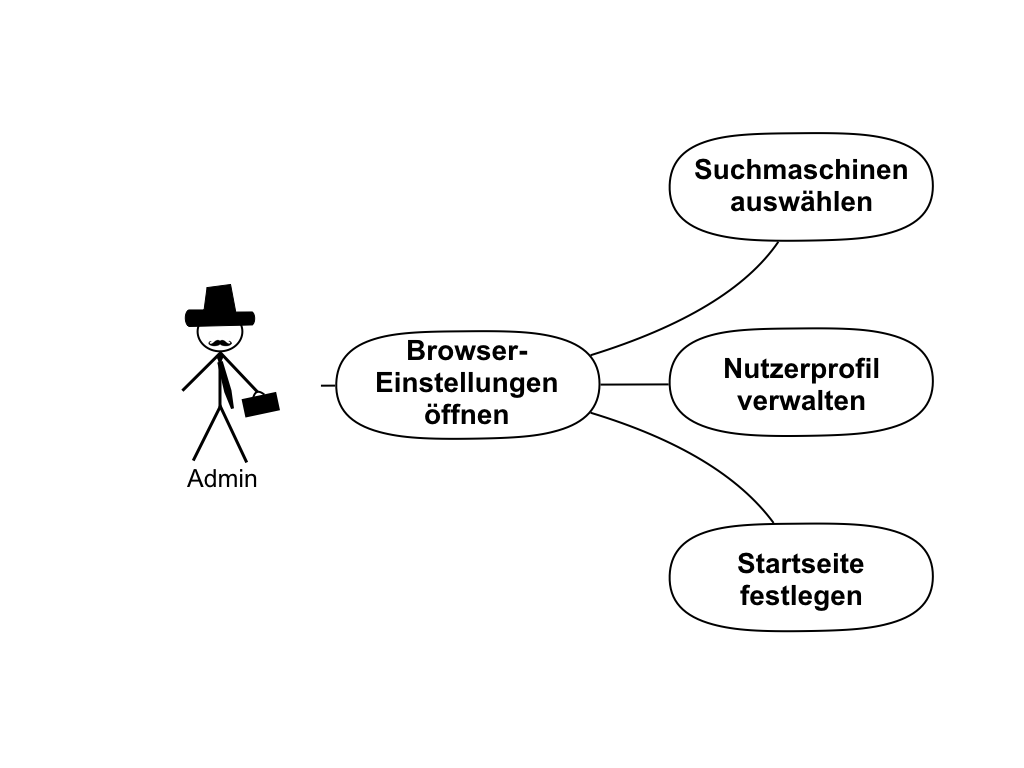
\includegraphics[width=\textwidth]{Use-Case-Diagramme_005.png}
	\caption{Use--Case--Diagramm --- Browser--Einstellungen}
	\label{fig:Browser-Einstellungen}
\end{figure}
Befindet sich der Nutzer in den Browser-Einstellungen, so hat er die Möglichkeit bestimmte Suchmaschinen, welche für die Suchergebnisse der \SEARCH-Tags verwendet werden, zu aktivieren oder diese zu deaktivieren. Im Weiteren kann der Benutzer sein persönliches Nutzerprofil verwalten und seine Startseite für die Applikation festlegen, welche direkt nach dem Öffnen der Anwendung als erste Seite geladen wird.
